\documentclass[11pt,journal,compsoc]{IEEEtran}

\usepackage[T1]{fontenc}
\usepackage[utf8]{inputenc}
\usepackage[french]{babel} % Global stuff set to french
\usepackage{tcolorbox}
\usepackage{amsmath, amssymb,  commath}

\begin{document}


\title{Open Wifi Localizator}
\author{Rémy Detobel, Denis Hoornaert, Nathan Liccardo, Robin Petit\\ Université libre de Bruxelles, Département des sciences informatiques, Bruxelles}

\maketitle

%\newpage

\begin{abstract}
  blablabla...
\end{abstract}
\begin{IEEEkeywords}
  Computer Society, IEEEtran, journal, \LaTeX, paper, template.
\end{IEEEkeywords}
\section{Introduction}
\section{Modélisation}
  \subsection{Graphe}
  \subsection{Recherche du plus court chemin}
    \subsubsection{A*}
    \subsubsection{Dijkstra}
\section{Localisation}
  \subsection{Introduction aux Wifi}
  \subsection{Problème rencontrer par l'utilisation des Wifi}
    Ce qui distingue la localisation via \textit{Wifi} des autres types de localisation est le caratère imprévisible de la propagation des ondes. En effet, bien que la propagation dans un espace ouvert suit une fonction donnée, la propagation des ondes au seins d'un batiment est plus complexe à cause de la reflexion de l'atténuantion des ondes survenant au contacte des murs. De plus, l'environement n'est pas la seule source d'altération du signal. En effet, un signal peut subir une déterioration de sa qualité de l'ordre de $-3.5 dBm$ si une personne se trouve entre l'émetteur et le recepteur(Mettre référence). Le signal peut aussi est déterioré par des interférences dont les sources peuvent être multiple. La difficulté repose dans ces deux derniers points car ceux-ci surviennent le plus souvent de manière inopinée.\\\\
    Pour avoir un moyen efficace de se localiser sur base des \textit{Wifi}, il faut pouvoir résoudre ces différents problèmes ou trouver un moyen de les rendre moins significatifs.
    \begin{center}
      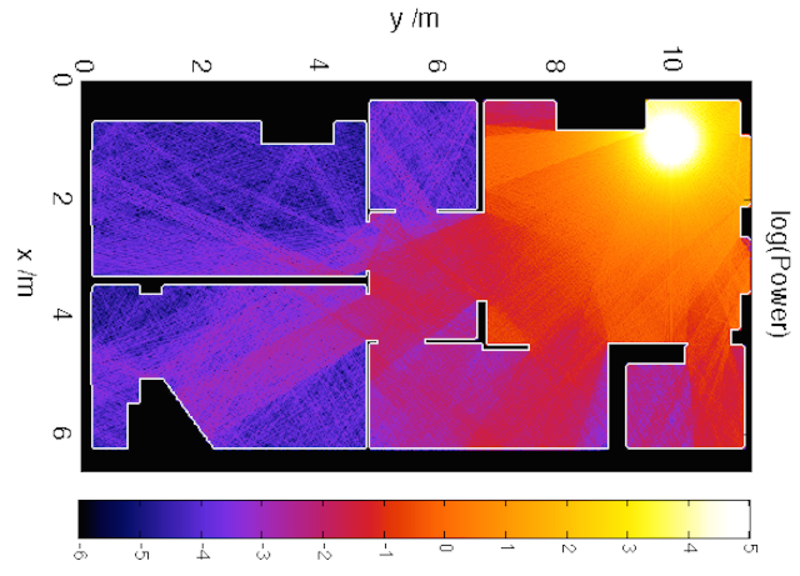
\includegraphics[scale=0.3]{images/wifi-propagation.png}
    \end{center}
  \subsection{Méthodes}
    On peut diviser les méthodes de localisation en deux catégories bien distinctes.\\
    Nous avons dans un premier temps, les méthodes dites de "propagation" qui se basent sur la connaissance préalable de l'ensemble des points d'accès \textit{Wifi} qui seront utilisés ainsi que sur la qualité du signal que reçoit l'utilisateur pour pouvoir déterminer la position exacte de ce dernier.\\
    Les méthodes de la deuxième catégorie parviennent, quand à elle, à localiser l'utilisateur en calculant la similarité entre une mesure (ensemble de \textit{Wifi}) donnée et une mesure présente en base de données et qui a été faite ultérieurement.\\
    Ces méthodes seront discutées et expliquées dans les deux sous-sections suivante.
    \subsubsection{Trilateration}
      La trilatération est une méthode mathématique permettant de trouver une coordonnée "concensus" qui sera contenu entre trois cercles. À la différence de la triangulation, la trilatration est basée sur l'utilisation de trois distances alors que la triangulation utilise trois angles donnés. Le schéma typique d'une trilatération est représenté par la figure ?.
      \begin{center}
        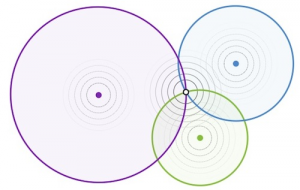
\includegraphics[scale=0.8]{images/trilateration.png}
      \end{center}
      Plus formallement, pour déterminer la position d'un utilisateur sur un plan cartésienne, nous devons bénéficier des coordonnées cartésiennes du centre de chaque cercle ainsi que de la distance entre l'utilisateur et ces centres comme mentionné plus haut. L'obtension des coordonnées cartésiennes de l'utilisateur sont obtenues via les formules suivante :
      \begin{equation}
        x = \frac{CE-BF}{EA-BD}
      \end{equation}
      \begin{equation}
        y = \frac{FA-DC}{EA-BD}
      \end{equation}
      Où :
      \begin{itemize}
        \item $A = 2x_{2}-2x_{1}$
        \item $B = 2y_{2}-2y_{1}$
        \item $C = r_{1}^{2}-r_{2}^{2}-y_{1}^{2}+y_{2}^{2}-x_{1}^{2}+x_{2}^{2}$
        \item $D = 2x_{3}-2x_{2}$
        \item $E = 2y_{3}-2y_{2}$
        \item $F = r_{2}^{2}-r_{3}^{2}-y_{2}^{2}+y_{3}^{2}-x_{2}^{2}+x_{3}^{2}$
      \end{itemize}
      (Voir annexe pour développement détailé)\\
      L'adaptation de la trilatération au problème de localisation se fait en déterminant la distance séparant l'utilisateur d'un point d'accés \textit{Wifi} (centre de cercles). On obtient la distance entre un recepteur (utilisateur) et un émetteur via une fonction qui prend en paramètre la qualité de signal de l'émetteur perçu par le recepteur. La fonction est la suivante :
      \begin{equation}
        \alpha_f(s) = \frac{27,55-20\log_{10}(f)+\abs s}{20}
      \end{equation}
      \begin{equation}
        d_f(s) = 10^{\alpha_f(s)}
      \end{equation}
      où :
      \begin{itemize}
        \item $f$ est la fréquence (généralement 2.4Ghz ou 5.0 GHz)~;
        \item $s$ est la qualité du signal (mesuré en $dBm$).
      \end{itemize}
      \begin{center}
        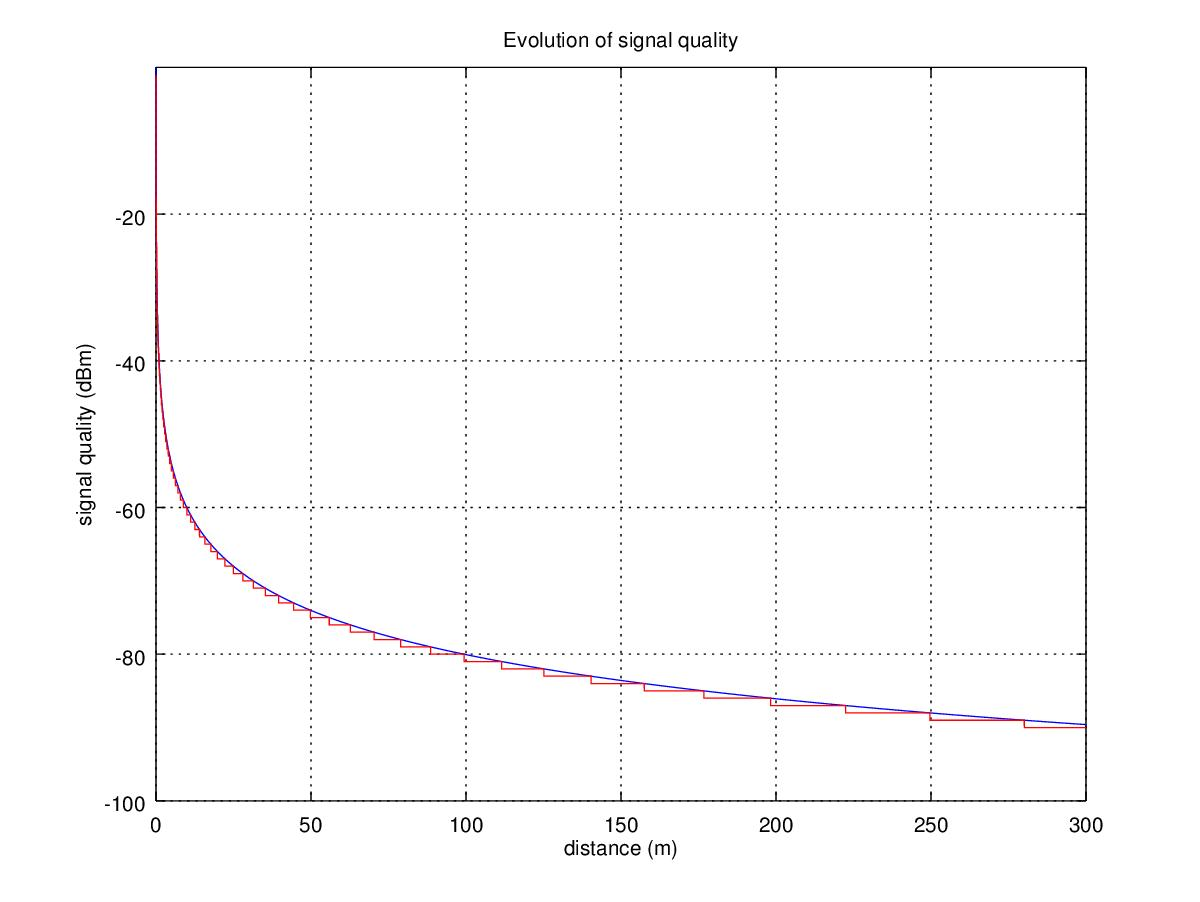
\includegraphics[scale=0.4]{images/signal-propagation.jpg}
        \textit{Répartition de la qualité de signal en fonction de la distance.}
      \end{center}
      L'utilisation d'une telle fonction donne de bon résultats dans un environement ouvert ou les obstacles sont rares. comme démontré par (Mettre référence) la précison de la localisation est situé entre x et y mètre. Néanmoins, dans le cas contraire, la fonction d'évaluation de la distance ne prenant pas en compte les obstacles, les estimations de distance s'en retrouvent biaisées et les coordonnées supposées de l'utilisateur aussi. De manière à résoudre ce problème, il est possible de remplacer la constante dans la formule (3) par une formule prenant en compte les éléments composant l'environement. Cette formule est définit comme suit :
      \begin{equation}
        \text{PLACER QQCH ICI}
      \end{equation}
      Cette modification de la trilatération implique de posséder encore plus de connaissance sur l'environement. Collecter ces données demande du temps et même en consentant à les collecter, les estimations de distance laissent à désiré.
    \subsubsection{Localisation via une Signal strength map}
      Une \textit{SSM} est défini comme étant une cartographie des régions couvertes par les signaux \textit{Wifi}. La construction de cette carte se fait en regardant et enregistrant quels sont les points d'accès \textit{Wifi} que l'on capte pour à une certaine position. On va donc enregistrer, dans une base de données, pour chaque position désirée, les identifiants (\textit{BSS}) et les qualités de signal des points d'accès \textit{Wifi} couvrant cette position.
      \paragraph{Méthode utilisant les processus Gaussiens}
      \paragraph{Méthode utilisant les maximum de vraisemblabilité}
        Comme mentionné plus haut, on va faire un ensemble de mesures pour chaque point du graphe et ainsi construtuire la base de données sur laquelle se basera notre méthode de localisation. Pour la méthode présente, on notera une mesure comme suit :
        \begin{equation}
          S^{(i)}=\{b_{1}, b_{2}, ..., b_{n}\} \hspace{1cm} \forall j \in [1, k]
        \end{equation}
        Où :
        \begin{itemize}
          \item $n$ est le nombre de points d'accès détectés lors de la mesure.
          \item $b_{i}$, le $i^{eme}$ point d'accès detécté, est défini comme un tuple $(a_{i}, S_{i})$ décrivant respectivement l'identifiant d'un point d'accès et la qualité de signal perçue.
        \end{itemize}
        
        On prend plusieurs mesures pour un même point car il existe des variations de qualité de signal au cour du temps. En faisant de la sorte, on se donne une idée de la qualité d'un signal à un point du graphe. On notera ces "mesures moyennes" comme suit :
        \begin{equation}
          \bar{S} = \{(a_{1}, \bar{S}_{1}), ..., (a_{n}, \bar{S}_{n})\}
        \end{equation}
        Où :
        \begin{itemize}
          \item $\bar{S}_{i} = \frac{1}{k}\sum\limits_{j = 1}^{k} S_{i}^{i} \hspace{1cm} \forall i \in [1, n]$
        \end{itemize}
        Cependant, considérer seulement la moyenne comme util statistique n'est pas suffisant due aux bruits et interférences pouvant survenir (voir section précédente). Pour pallier à ce problème, on cacule aussi la variance (noté $v$) pour chaque point du graphe. Ainsi, on obtiendra une nouvelle forme appellée ensemble charactéristique qui est définit comme suit :
        \begin{equation}
          S^{*} = \{(a_{1}, \bar{S}_{1}, v_{1}), ..., (a_{n}, \bar{S}_{n}, v_{n})\}
        \end{equation}
        Où :
        \begin{itemize}
          \item $v_{i} = \frac{1}{k-1}\sum\limits_{j = 1}^{k}(S_{i}^{(j)}-\bar{S}_{i}) \hspace{1cm} \forall i \in [1,n]$
        \end{itemize}
        On peut donc définir notre base de données (notée $\mathcal{D}$) comme l'ensemble des points du graphe (noté $L$) pour lequel il existe un ensemble charactéristique. Soit : 
        \begin{equation}
          \mathcal{D} = \{L_{1}, L_{2}, ..., L_{3}\}
        \end{equation}
        Où :
        \begin{itemize}
          \item $\dim(L_{i})$, le nombre de points d'accès à cette position, est noté $n_{i}$
          \item $S_{i}^{*}$ est l'ensemble charactéristique de $L_{i}$ 
        \end{itemize}
        
        Une fois la base de données remplie, on peut passer à l'étape dites d'exploitation. Il s'aggit du processus qui sera utilisé par une personne pour pouvoir se localiser.\\
        Le processus va déduire la position de l'utilisateur sur base de la base de données préalablement crée (notée $\mathcal{D}$) et sur base d'une mesure qu'il aura effectuée (notée $S'$). La nature de cette mesure pouvant soit être de la forme (1) ou (2).\\
        Le processus va déterminer une position $\hat{L}$ appartenant $\mathcal{D}$ pour laquelle la probabilité que l'utilisateur se trouve proche de ce point est la plus grande. Pour se faire, on va calculer, pour chaque élément appartenant à $\mathcal{D}$, un score noté $Z$ et considérer, comme solution à notre problème, le point conrespondant au score $Z$ minimal car le score $Z$ minimal représent la vraisemblabilité maximale comme prouvé dans l'article (Mettre référence). Le score $Z$ est définit comme suit :
        \begin{equation}
          Z_{i} = \sum\limits_{j = 1}^{n_{i}}\bigg(\frac{(\bar{S}_{ij}-S'_{j})^{2}}{v_{ij}}\bigg)
        \end{equation}
        Où :
        \begin{itemize}
          \item $\bar{S}_{ij}$ est la moyenne de la qualité de signal du $j^{eme}$ point d'accès
          \item $v_{ij}$ est la variance de la qualité de signal du $j^{eme}$ point d'accès
          \item $S'_{j}$ est la qualité de signal du $j^{eme}$ point d'accès de la mesure effectué par l'utilisateur
        \end{itemize}
        
        \begin{tcolorbox}[title = Mesures parasites]
          Dans cette article, on défini une mesure parasite comme la détection d'un point d'accès qui n'apparaitrait que très rarement lors de la prise de mesures. On qualifira un point d'accès comme tel si le nombre de fois qu'il a été détecté est inférieur à un seuil fixé.
          \\
          Ce cas de figure survient pour des points d'accès situés à une distance telle qu'ils ne sont pas toujours percus mais qui, dans le cas contraire, présentent des qualités de signal in férieur à $-90 dBm$.
        \end{tcolorbox}
      \paragraph{Monte carlo}
      \paragraph{Amélioration par l'utilisation de filtres}
      \paragraph{Amélioration par l'estimation de qualité de signal}
\section{Discussion et limitations}
\section{Conclusion}

\begin{thebibliography}{9}
  \bibitem{ssm}
    Matteo Cypriani, Frédéric Lassabe, Philippe Canalda, François Spies,
    \emph{Wi-Fi-Based Indoor Positioning: Basic Techniques, Hybrid Algorithms and Open Software Platform}.
    2010.
  \bibitem{Roumanie}
    Bianca BOBESCU, Marian ALEXANDRU
    \emph{Mobile indoor positioning using Wi-fi localisation}.
    Transilvania University, Brasov, Romania,
    2015.
  \bibitem{trilateration}
    OnkarPathak, Pratik Palaskar, Rajesh Palkar, Mayur Tawari,
    \emph{Wi-Fi Indoor Positioning System based on RSSI Measurements from Wi-Fi Access Points A Trilateration Approach}.
    International Journal of Scientific \& Engineering Research,
    2014.
  \bibitem{GaussianProcessesFerris}
    Brian Ferris, Dirk Hähnel, Dieter Fox,
    \emph{Gaussian Processes for Signal Strength-Based Location Estimation}.
    University of Washington, Department of Computer Science \& Engineering, Seattle, WA Intel Research Seattle, Seattle, WA.
\end{thebibliography}

%---------- SCANNING ----------
%# www.mdpi.com/1424-8220/15/9/21824/pdf
%https://www.researchgate.net/publication/224198838_Wi-Fi-based_indoor_positioning_Basic_techniques_hybrid_algorithms_and_open_software_platform
%x https://fruct.org/publications/abstract16/files/Shc1.pdf
%http://www.afahc.ro/ro/revista/2015_1/119.pdf
%x http://file.scirp.org/pdf/CN_2013071010352139.pdf
%http://www.ijser.org/researchpaper%5CWi-Fi-Indoor-Positioning-System-Based-on-RSSI-Measurements.pdf
%https://www.researchgate.net/profile/Suhailan_Safei/publication/230771403_INDOOR_POSITION_DETECTION_USING_WIFI_AND_TRILATERATION_TECHNIQUE/links/5513e9120cf2eda0df3031f0.pdf
%http://www.ee.ucl.ac.uk/lcs/previous/LCS2005/12.pdf
%http://www.int-arch-photogramm-remote-sens-spatial-inf-sci.net/XXXVIII-4-C26/1/2012/isprsarchives-XXXVIII-4-C26-1-2012.pdf
%---------- LOCALISATION ----------
%http://www.roboticsproceedings.org/rss02/p39.pdf
%https://venturi.fbk.eu/wp-content/uploads/2011/10/AraMes_WIMOB_2014.pdf
%http://www.tik.ee.ethz.ch/file/2490a7adb6a163b9c5be1510d033870a/sawn05.pdf
%https://felixduvallet.github.io/pubs/2008-WiFi-IROS.pdf
%http://www.cs.cmu.edu/~mmv/papers/10icra-joydeep.pdf
%https://papers.nips.cc/paper/2541-gpps-a-gaussian-process-positioning-system-for-cellular-networks.pdf
%http://www-cs.stanford.edu/people/dstavens/icra11/huang_etal_icra11.pdf
%https://www.ncbi.nlm.nih.gov/pmc/articles/PMC5017359/
%http://www.robot.t.u-tokyo.ac.jp/~yamashita/paper/E/E293Final.pdf

\section*{Annexes}

\end{document}
